\documentclass{article}

\usepackage[a4paper]{geometry}
\usepackage[spanish]{babel}
\usepackage{xcolor}
\usepackage{placeins}

\usepackage{mathbbol}
\usepackage{amsmath}
\usepackage{amsfonts}
\usepackage{hyperref}
\usepackage{graphicx}
\usepackage{subcaption}

\usepackage{algorithm}
\usepackage{algpseudocode}

% Cambiar 'Cuadro' -> 'Tabla'
\addto\captionsspanish{
    \renewcommand{\tablename}{Tabla}
}

\begin{document}

\begin{center}
    {\Large Aprendizaje Automático para Datos en Grafos} \\
    {\LARGE \textbf{Laboratorio 4}} \\
    \vspace{2em}
    \begin{minipage}{0.45\textwidth}
        \centering
        Graciana Castro \\
        4.808.848-2 \\
        gcastro@fing.edu.uy
    \end{minipage}
    \hfill
    \begin{minipage}{0.45\textwidth}
        \centering
        Julian O'Flaherty \\
        6.285.986-9 \\
        julian.o.flaherty@fing.edu.uy
    \end{minipage}
\end{center}


\section{Introducción}
Este informe presenta el Laboratorio 4 para la materia Aprendizaje Automático para Datos en Grafos. El objetivo principal es abordar el problema de inferencia de topología en grafos, es decir, la estimación de la estructura subyacente (aristas y pesos) de un grafo a partir de observaciones o medidas en sus nodos. Este problema es fundamental en muchas aplicaciones reales donde se conocen los nodos de una red pero no las conexiones entre ellos, y solo se dispone de señales o características observadas en cada nodo.

Se exploran tres metodologías principales: Graphical Lasso (Friedman, Hastie y Tibshirani, 2008), Meinshausen y Bühlmann (2006) y Kalofolias (2016). En la primera parte, descrita en la sección \ref{sec:datos_sinteticos}, se aplican estos métodos sobre datos sintéticos para evaluar su capacidad de recuperar estructuras conocidas. La segunda parte, sección \ref{sec:mnist}, utiliza el dataset MNIST de dígitos manuscritos, donde cada imagen se interpreta como un nodo del grafo y se evalúa el desempeño mediante clustering espectral. El código implementado puede consultarse en el repositorio de GitHub \url{https://github.com/j-oflaherty/AA-grafos/blob/main/lab4/Lab4_AAG2025.ipynb}.



\section{Inferencia de topología en datos sintéticos}
\label{sec:datos_sinteticos}

\subsection{Generación del grafo sintético}

Para generar un grafo sintético, utilizaremos el siguiente algoritmo:
\begin{enumerate}
    \item Sorteamos $N$ puntos de forma uniforme en el cuadrado $[0,1] \times [0,1]$. Esos serán los vértices de nuestro grafo.
    \item Para cada par de puntos $i$ y $j$ que sorteamos antes, tomamos como peso de la arista
    \begin{equation*}
        w_{ij} = \begin{cases}
            0 & \text{si } i=j \\
            e^{-\frac{d(i,j)}{2\sigma^2}} & \text{si } i \neq j
        \end{cases}
    \end{equation*}
    donde $d(i,j)$ es la distancia euclidea en $\mathbb{R}^2$ y $\sigma$ es un parámetro fijo.
    \item Descartamos las aristas cuyo peso $w_{ij}$ sea menor que un número fijo $r>0$.
\end{enumerate}
En la figura~\ref{fig:grafo_sintetico} se muestra un grafo sintético generado con el algoritmo anterior para $N=50$, $\sigma=0.5$ y $r=0.6$.

\begin{figure}[htb]
    \centering
    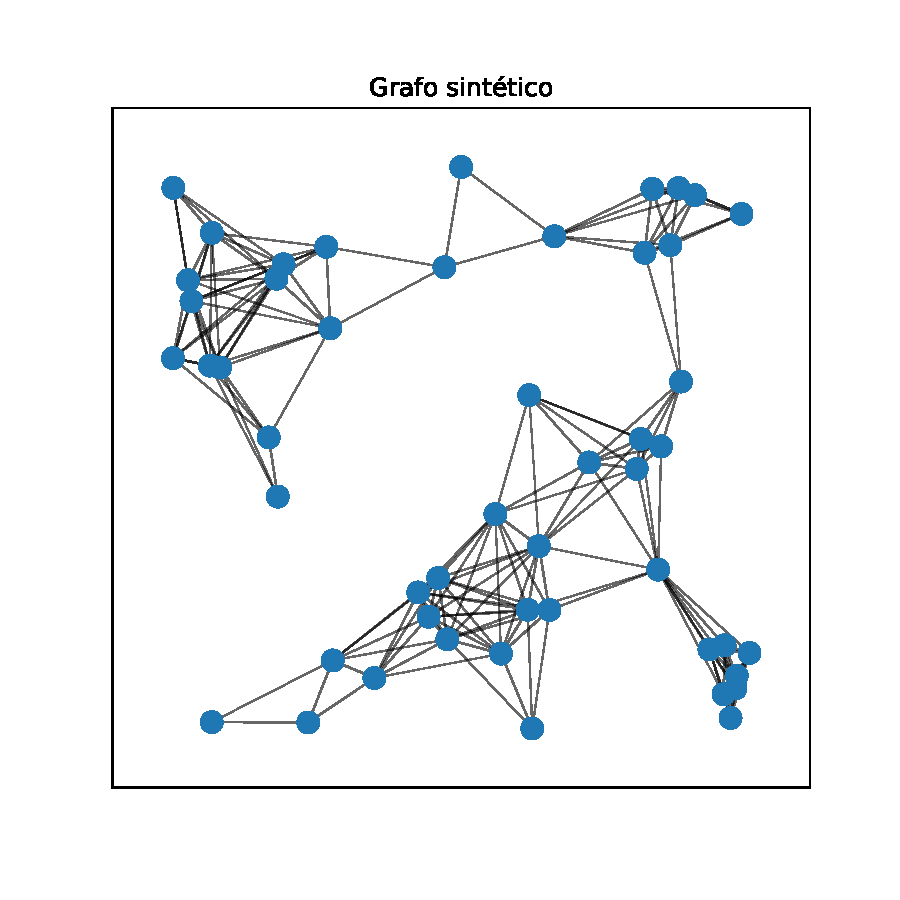
\includegraphics[width=0.5\textwidth]{imagenes/grafo_sintetico.pdf}
    \caption{Grafo sintético generado con $N=50$, $\sigma=0.5$ y $r=0.6$.}
    \label{fig:grafo_sintetico}
\end{figure}

A cada nodo del grafo sintetico, le asignaremos una señal $x_i \sim \mathcal{N}(0, \mathbf{L}^\dagger)$, donde $\mathbf{L}^\dagger$ es la pseudoinversa de la matriz laplaciana $\mathbf{L}$ del grafo. En la figura~\ref{fig:signals_X_pseudoinverse} se muestra un \textit{sample} de señales
donde cada columna $j$ es la señal asociada al nodo $j$ del grafo. La cantidad de filas, o el tamaño de la muestra, es el parámetro $n_{\text{samples}}$ del algoritmo, por lo que si $n_{\text{samples}}$ es menor que $N$, la matriz de covarianza empírica no es invertible.

\begin{figure}[htb]
    \centering
    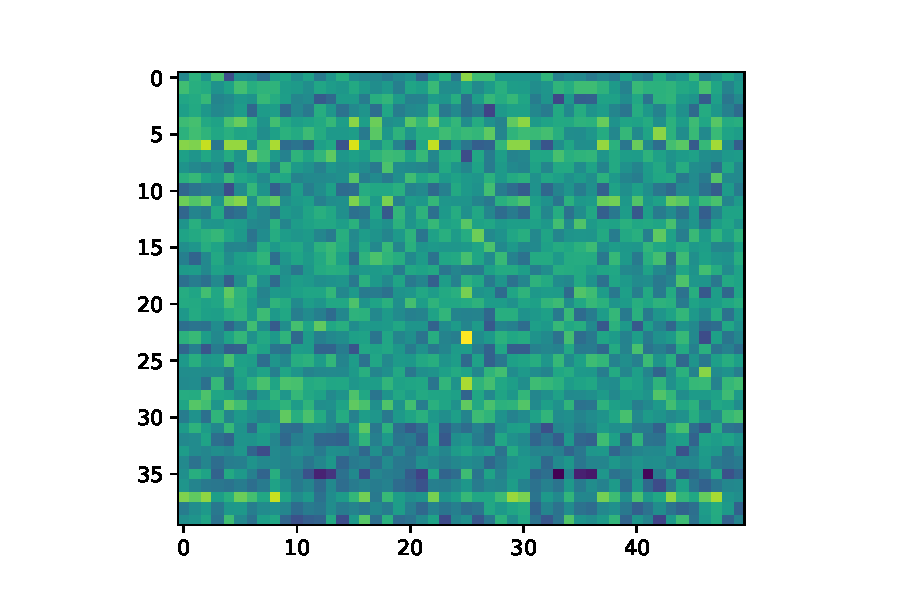
\includegraphics[width=0.6\textwidth]{imagenes/signals_X_pseudoinverse.pdf}
    \caption{Sample de señales asignadas a los nodos del grafo sintético.}
    \label{fig:signals_X_pseudoinverse}
\end{figure}

\subsection{Estimación de estructura con Graphical Lasso}

Estimaremos la estructura del grafo a partir de la matriz de datos utilizando el método \textit{Graphical Lasso}. Este método busca al estimador 
de máxima verosimilitud de la matriz de precisión $\boldsymbol{\Theta}$ que cumple:
\begin{equation}
\hat{\boldsymbol{\Theta}} = \arg \max_{\boldsymbol{\Theta} \succeq 0} \left\{ \log \det \boldsymbol{\Theta} - \text{trace}(\hat{\boldsymbol{\Sigma}} \boldsymbol{\Theta}) - \lambda \|\boldsymbol{\Theta}\|_1 \right\}
\end{equation}
Una de las propiedades importantes del Graphical Lasso, es que cuando $\lambda =  2\sqrt{\frac{\log N}{P}}$,
\begin{equation*}
    \|\hat{\boldsymbol{\Theta}} - \boldsymbol{\Theta}_0\|_2 \leq \sqrt{\frac{d_{\max}^2 \log N}{P}} \quad \text{w.h.p.}
\end{equation*}

con el parámetro $\lambda$ siendo parámetro de regularización. 
\begin{figure}[htb]
    \centering
    \begin{subfigure}[t]{0.32\linewidth}
        \centering
        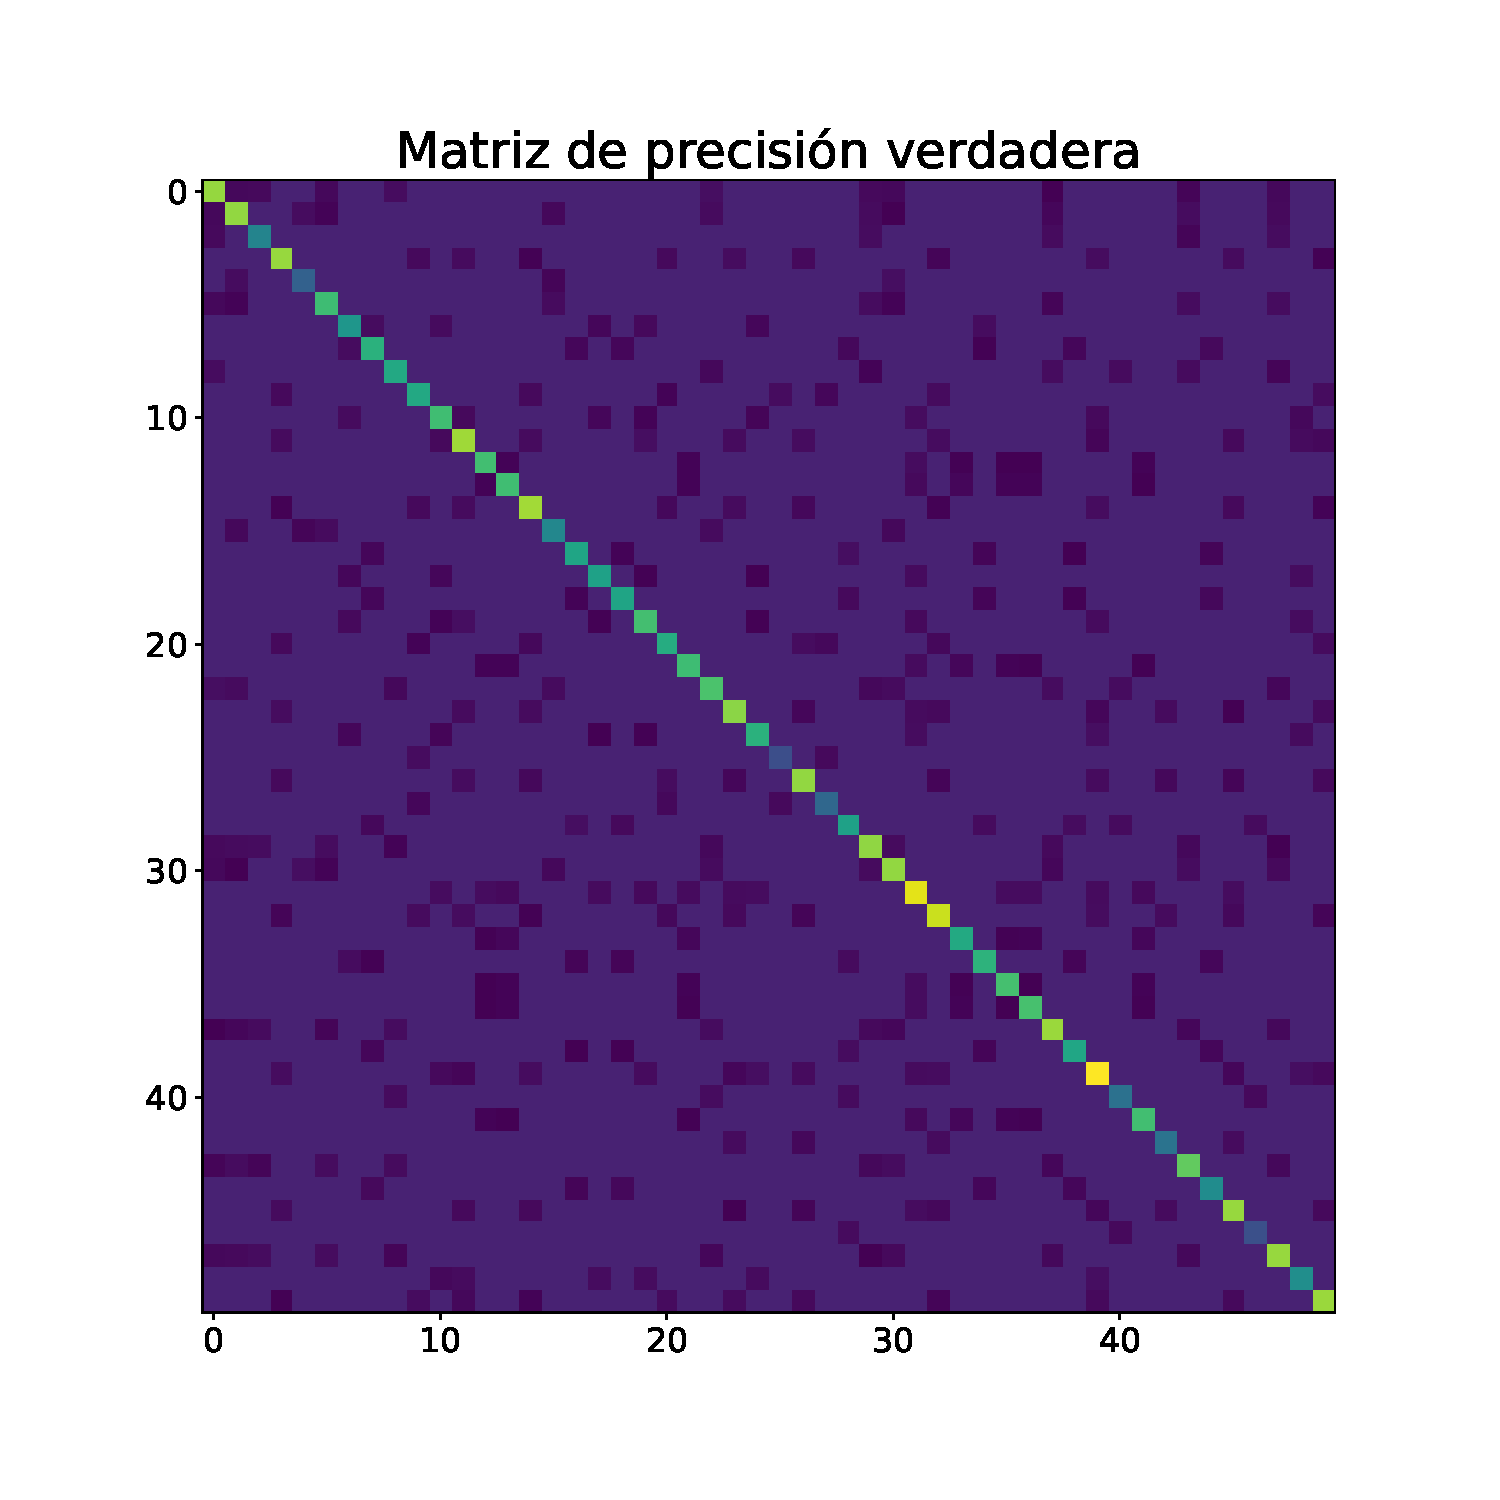
\includegraphics[width=\textwidth]{imagenes/graphical_lasso/true_precision_sample.pdf}
        \caption{Precisión verdadera}
        \label{fig:graphical_lasso_true_precision}
    \end{subfigure}\hfill
    \begin{subfigure}[t]{0.32\linewidth}
        \centering
        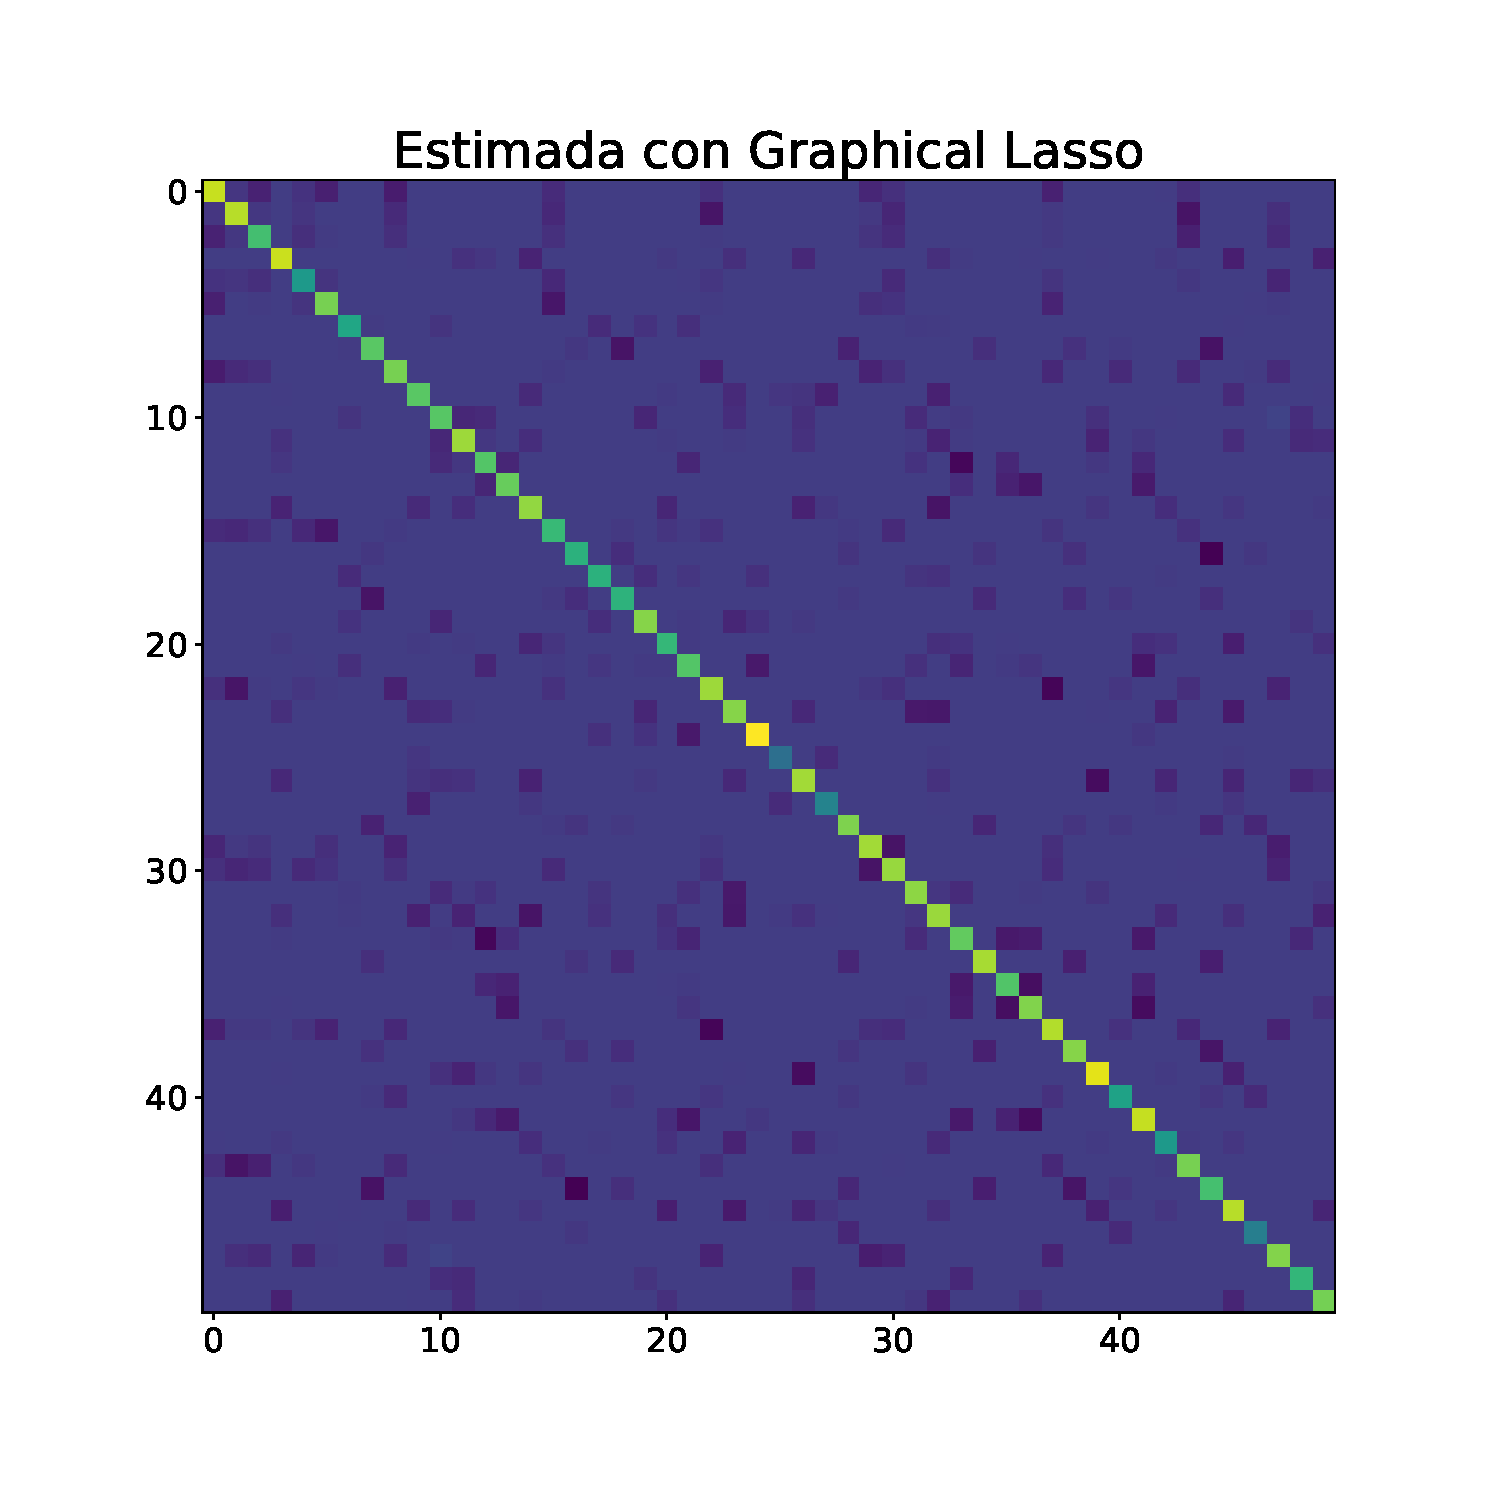
\includegraphics[width=\textwidth]{imagenes/graphical_lasso/graphical_sample.pdf}
        \caption{Estimación mediante Graphical Lasso}
    \end{subfigure}\hfill
    \begin{subfigure}[t]{0.32\linewidth}
        \centering
        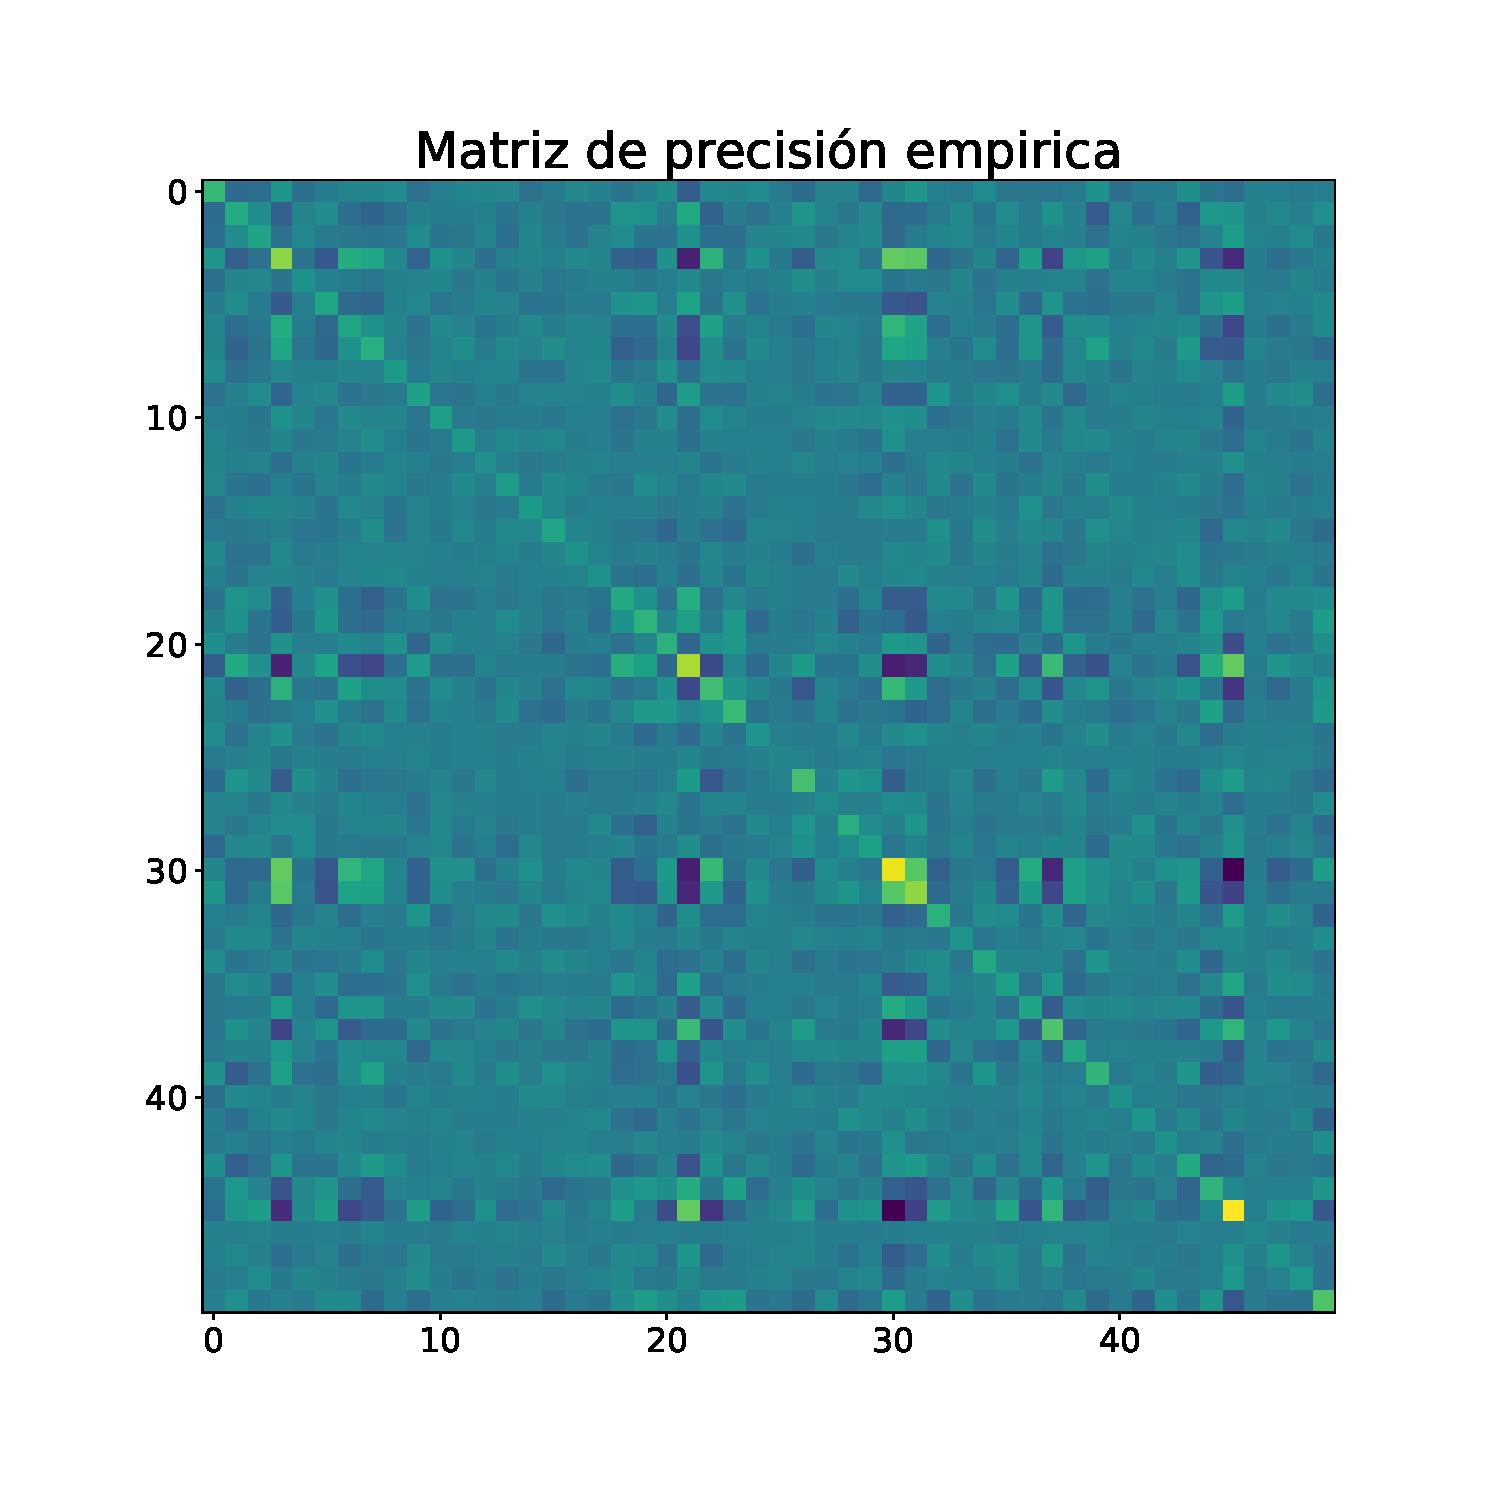
\includegraphics[width=\textwidth]{imagenes/graphical_lasso/estimated_sample.pdf}
        \caption{Estimación empírica \\ ($\Theta = \Sigma^{-1}$)}
    \end{subfigure}
    \caption{Comparación entre la matriz de precisión verdadera, la estimación mediante Graphical Lasso y la estimación obtenida con empíricamente ($\Theta = \Sigma^{-1}$), cuando $n_{\text{samples}}=40$ y $N=50$}
    \label{fig:graphical_lasso_triptych}
\end{figure}
En la figura~\ref{fig:graphical_lasso_triptych} se puede observar la estimación obtenida con \emph{Graphical Lasso} comparada con la estimación empírica cuando el número de samples utilizado $n_{\text{samples}}$ es menor que la cantidad de nodos $N$. En este caso, la estimación
empírica resulta mala, dado que la matriz de covarianza empírica no es invertible. El método de \emph{Graphical Lasso} obtiene un resultado muy similar a la matriz de precisión verdadera, donde el valor de $\lambda$ se calcula mediante validación cruzada. 

En la figura~\ref{fig:graphical_lasso_alpha_comparison} observamos el efecto del variar el valor de $\lambda$ sobre la matriz de precisión estimada. A medida que aumenta la regularización, la matriz va perdiendo ceros tendiendo a una matriz diagonal, lo cual es esperable
dado que el valor de $\lambda$ está asociado a la norma 1 de la matriz de precisión.
\begin{figure}[htb]
    \centering
    \begin{subfigure}[t]{0.32\linewidth}
        \centering
        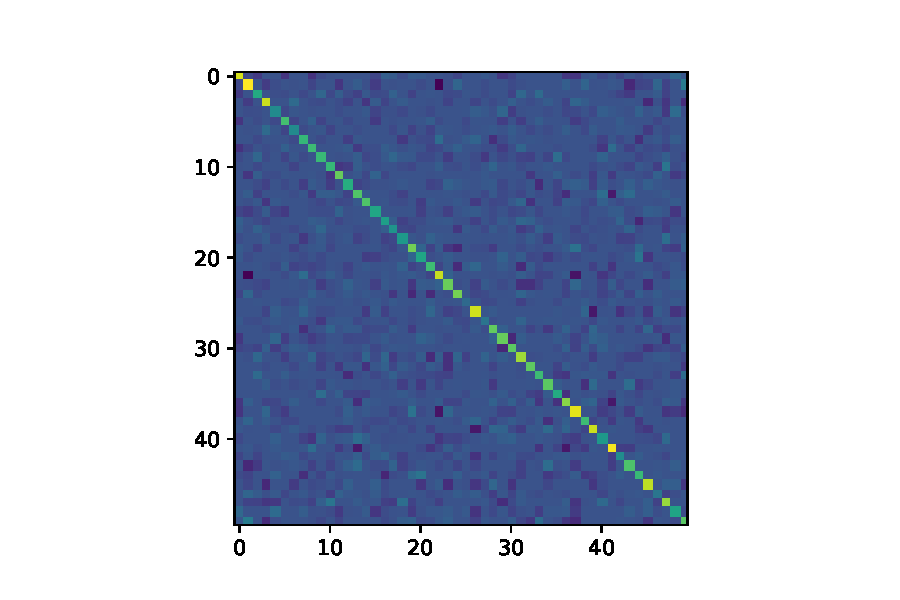
\includegraphics[width=\textwidth]{imagenes/graphical_lasso/graphical_lasso_alpha_0_01.pdf}
        \caption{$\lambda = 0.01$}
    \end{subfigure}\hfill
    \begin{subfigure}[t]{0.32\linewidth}
        \centering
        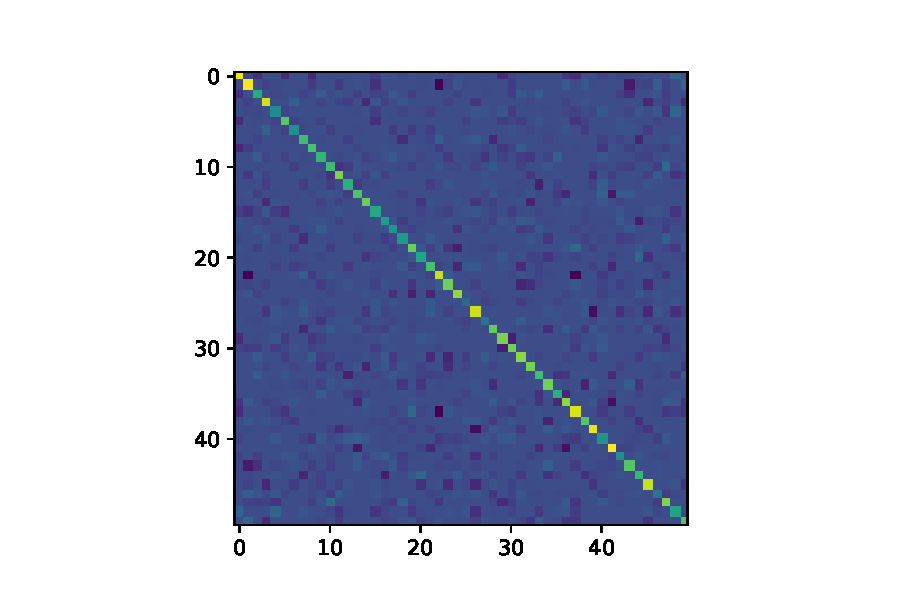
\includegraphics[width=\textwidth]{imagenes/graphical_lasso/graphical_lasso_alpha_0_02.pdf}
        \caption{$\lambda = 0.02$}
    \end{subfigure}\hfill
    \begin{subfigure}[t]{0.32\linewidth}
        \centering
        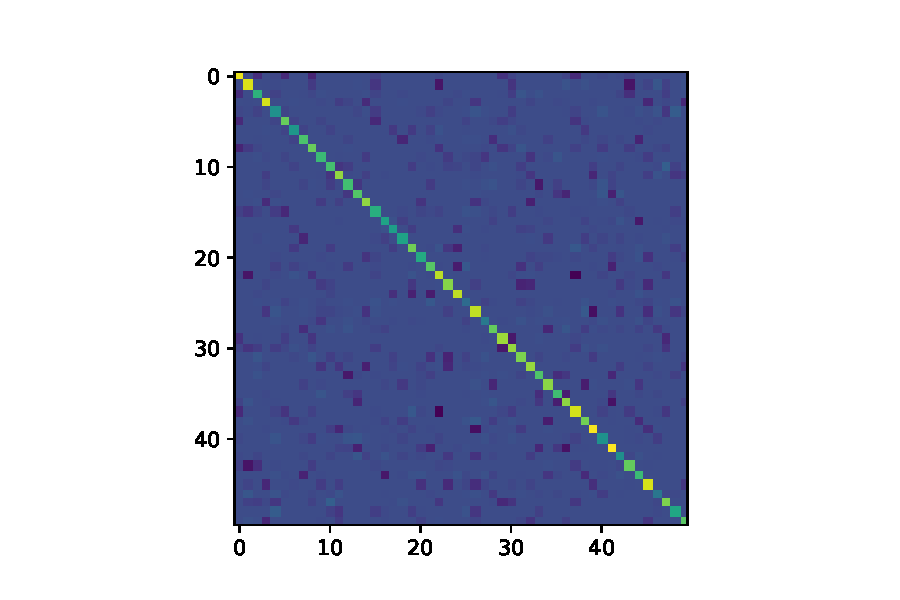
\includegraphics[width=\textwidth]{imagenes/graphical_lasso/graphical_lasso_alpha_0_05.pdf}
        \caption{$\lambda = 0.05$}
    \end{subfigure}
    \begin{subfigure}[t]{0.32\linewidth}
        \centering
        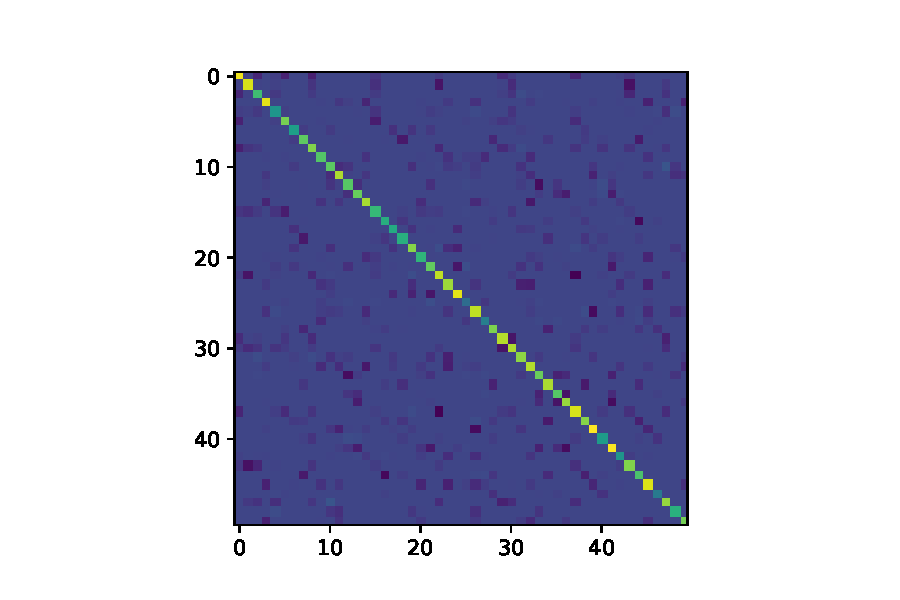
\includegraphics[width=\textwidth]{imagenes/graphical_lasso/graphical_lasso_alpha_0_1.pdf}
        \caption{$\lambda = 0.1$}
    \end{subfigure}
    \begin{subfigure}[t]{0.32\linewidth}
        \centering
        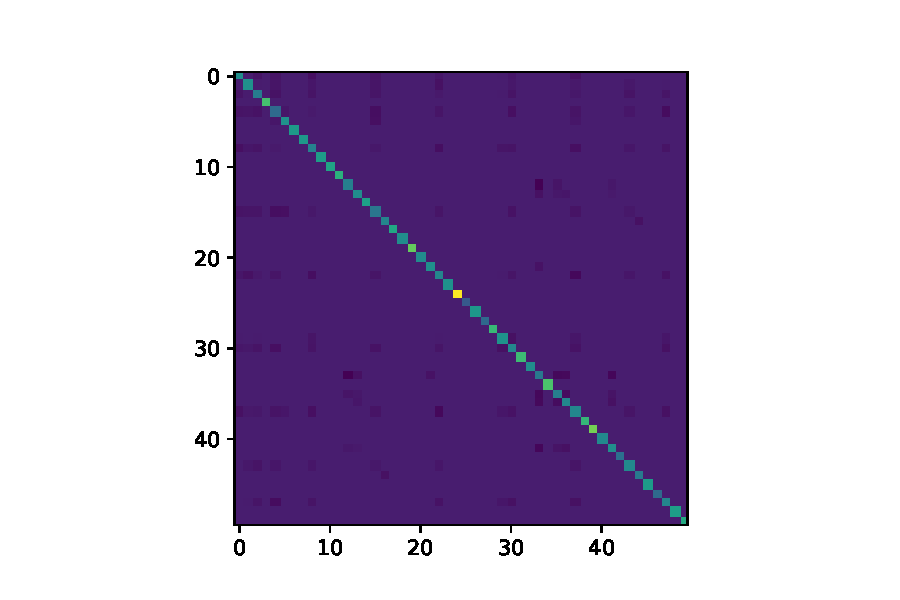
\includegraphics[width=\textwidth]{imagenes/graphical_lasso/graphical_lasso_alpha_0_5.pdf}
        \caption{$\lambda = 0.5$}
    \end{subfigure}
    \begin{subfigure}[t]{0.32\linewidth}
        \centering
        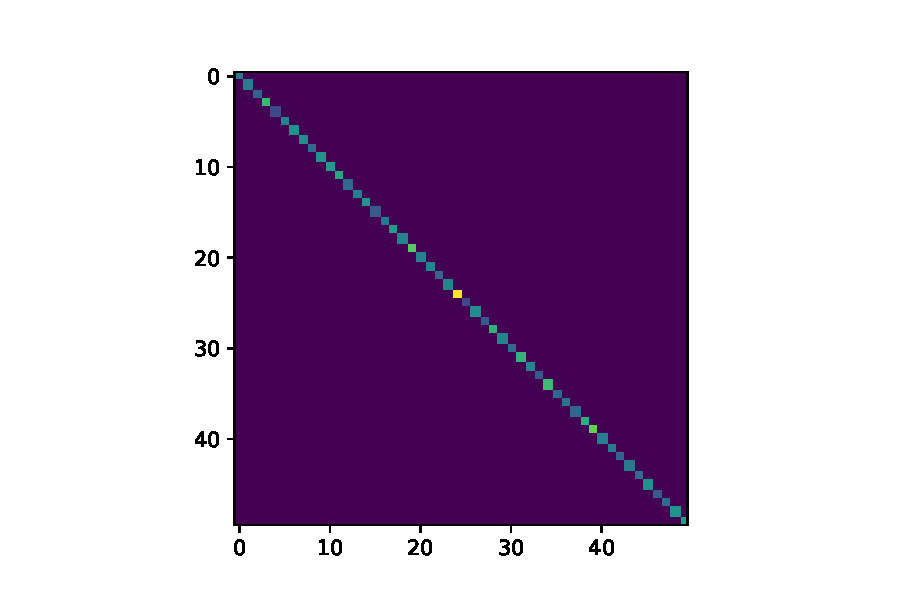
\includegraphics[width=\textwidth]{imagenes/graphical_lasso/graphical_lasso_alpha_1.pdf}
        \caption{$\lambda = 1$}
    \end{subfigure}
    \caption{Estimación mediante Graphical Lasso para distintos valores de $\lambda$. La matriz de precisión verdadera se muestra en la figura~\ref{fig:graphical_lasso_true_precision}. No se muestran valores menores a $0.01$ porque hay poca diferencia notable, y a partir de $0.005$ el sistema queda mal condicionado y no puede ser resuelto.
}
    \label{fig:graphical_lasso_alpha_comparison}
\end{figure}

\subsection{Estimación de estructura con Meinshausen y Bühlmann}

\subsection{Estimación de estructura con Meinshausen y Bühlmann}

El método de Meinshausen y Bühlmann propone una alternativa eficiente para la estimación de la estructura de grafos mediante selección de vecindarios con Lasso. Este método es particularmente útil en problemas de alta dimensionalidad donde $p \gg n$, ya que permite identificar los ceros estructurales en la matriz de precisión que representan restricciones de independencia condicional entre variables.

La idea central consiste en estimar el vecindario de cada nodo de forma individual mediante regresión. Para cada nodo $a$, se define su vecindario como el conjunto mínimo de variables que, al ser conocidas, hacen que $X_a$ sea condicionalmente independiente del resto. Esto se formula como un problema de regresión Lasso donde $X_a$ es la variable respuesta y las demás son predictoras:

\begin{equation}
    \hat{\theta}_{a,\lambda} = \operatorname*{argmin}_{\theta : \theta_a=0} \left(n^{-1}\|X_a - X\theta\|_2^2 + \lambda\|\theta\|_1\right)
\end{equation}

El vecindario estimado de $a$ se determina por los coeficientes no nulos de $\hat{\theta}_{a,\lambda}$. Una vez obtenidos todos los vecindarios, el conjunto de aristas del grafo se construye mediante la regla AND:

\begin{equation}
    \hat{E}_{\lambda, \wedge} = \{(a, b) : a \in \hat{n}e_{\lambda, b} \land b \in \hat{n}e_{\lambda, a}\}
\end{equation}

Una propiedad importante de este método es que mantiene consistencia incluso cuando $p \gg n$, siempre que el parámetro $\lambda$ se elija adecuadamente.

Para implementar este método, seguimos el siguiente algoritmo:
\begin{enumerate}
    \item Normalizamos la matriz de datos $\mathbf{X}$ por columnas.
    \item Inicializamos una matriz $\mathbf{B}$ de ceros de tamaño $p \times p$.
    \item Para cada nodo $j$ del grafo:
    \begin{enumerate}
        \item Extraemos la columna $j$ de $\mathbf{X}$ como variable objetivo $\mathbf{y}_j$.
        \item Utilizamos las demás columnas como matriz de predictores $\mathbf{X}_j$.
        \item Resolvemos el problema de regresión Lasso para obtener los coeficientes $\hat{\boldsymbol{\theta}}_j$.
        \item Insertamos los coeficientes en la fila $j$ de $\mathbf{B}$, colocando un cero en la posición $j$.
    \end{enumerate}
    \item Devolvemos la matriz $\mathbf{B}$ que contiene los coeficientes de regresión para cada nodo.
\end{enumerate}

En la figura \ref{fig: meinhausen} se observa que el método de Meinshausen y Bühlmann logra capturar la estructura principal de la matriz de coeficientes verdadera, identificando correctamente las conexiones más relevantes. Sin embargo, aparecen algunos falsos positivos y negativos, lo que refleja el compromiso entre detección y ruido inherente al uso de Lasso.

\begin{figure}[htb]
    \centering
    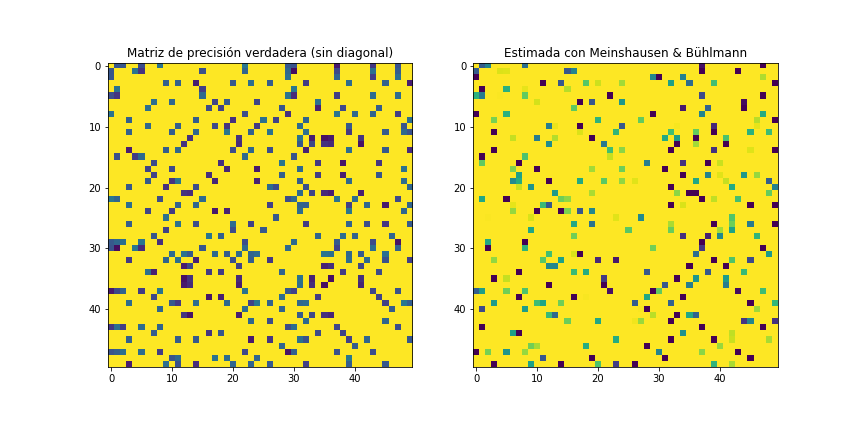
\includegraphics[width=0.6\textwidth]{imagenes/meinhausen/matriz_estimada.png}
    \caption{Comparación entre la matriz de coeficientes verdadera y la matriz de coeficientes estimada con el método de Meinshausen y Bühlmann.}
    \label{fig: meinhausen}
\end{figure}

\subsection{Estimación de estructura con Kalofolias}
El método propuesto por Kalofolias plantea aprender la estructura de un grafo a partir de señales que residen en sus nodos, asumiendo que estas señales cambian suavemente entre nodos conectados. La contribución clave consiste en reformular el problema tradicional de minimización del término de suavidad $\text{tr}(X^T L X)$ mostrando que es equivalente a una norma $\ell_1$ ponderada aplicada a la matriz de adyacencia $W$:

\begin{equation}
\text{tr}(X^T L X) = \frac{1}{2} \|W \circ Z\|_{1,1}
\end{equation}

donde $Z_{i,j} = \|x_i - x_j\|_2$ es la matriz de distancias por pares entre las señales. Esta equivalencia permite formular el problema de aprender el grafo como:

\begin{equation}
\min_{W \in \mathcal{W}_m} \|W \circ Z\|_{1,1} - \alpha \mathbf{1}^T \log(W \mathbf{1}) + \beta \|W\|_F^2
\end{equation}

El término logarítmico $-\alpha \mathbf{1}^T \log(W \mathbf{1})$ actúa sobre el vector de grados de los nodos, promoviendo la conectividad del grafo, mientras que el término $\beta \|W\|_F^2$ controla la dispersión de los pesos. Los parámetros $\alpha > 0$ y $\beta \geq 0$ permiten balancear estos objetivos.

En la figura \ref{fig:kalofolias_grid} se presentan los resultados obtenidos con diferentes combinaciones de $\alpha$ y $\beta$, comparados con la matriz verdadera. Se aprecia cómo estos parámetros influyen en la estructura del grafo aprendido, permitiendo ajustar el balance entre conectividad y dispersión de pesos según las características deseadas.

\begin{figure}[htb]
    \centering
    \begin{minipage}[t]{0.25\textwidth}
        \centering
        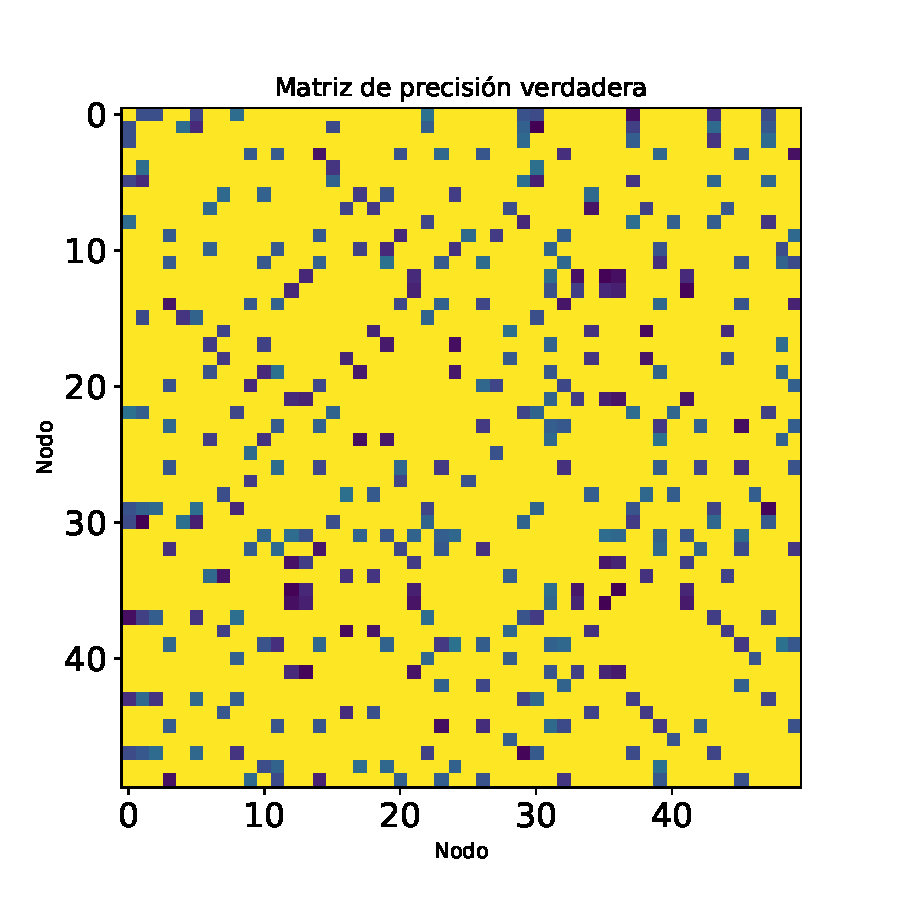
\includegraphics[width=\textwidth]{imagenes/kalofolias/kalofolias_true.pdf}
        \caption*{Matriz verdadera}
    \end{minipage}
    \hfill
    \begin{minipage}[t]{0.72\textwidth}
        \centering
        \begin{tabular}{ccc}
            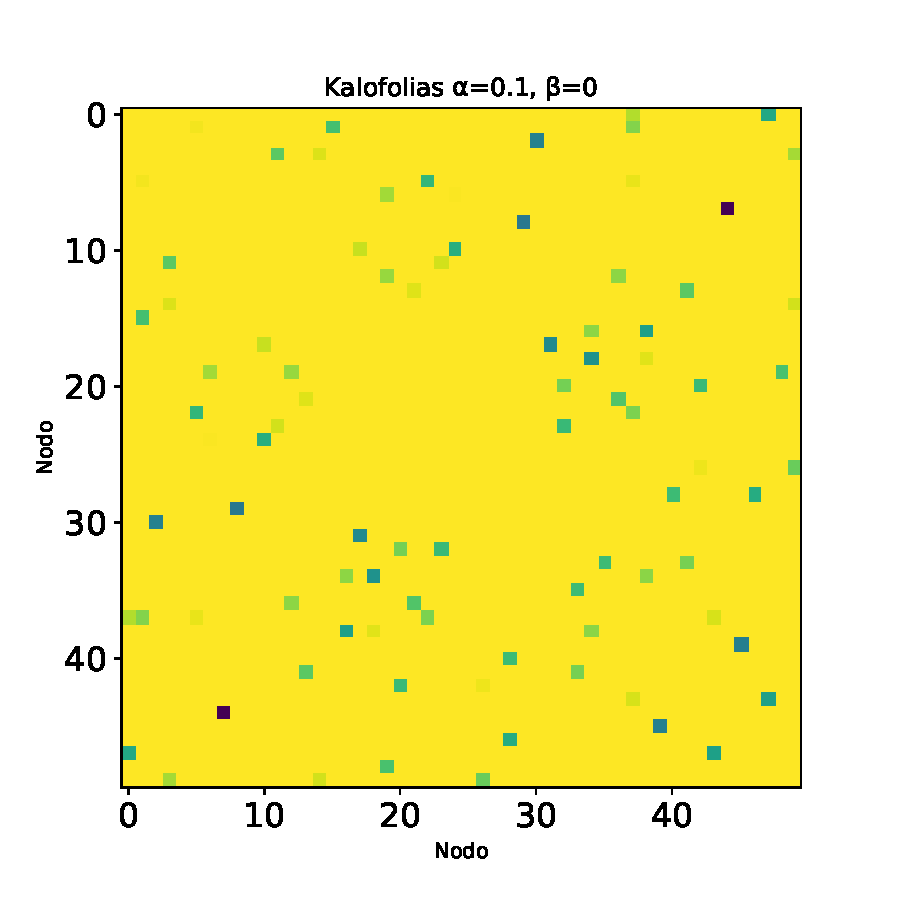
\includegraphics[width=0.28\textwidth]{imagenes/kalofolias/kalofolias_alpha0.1_beta0.pdf} &
            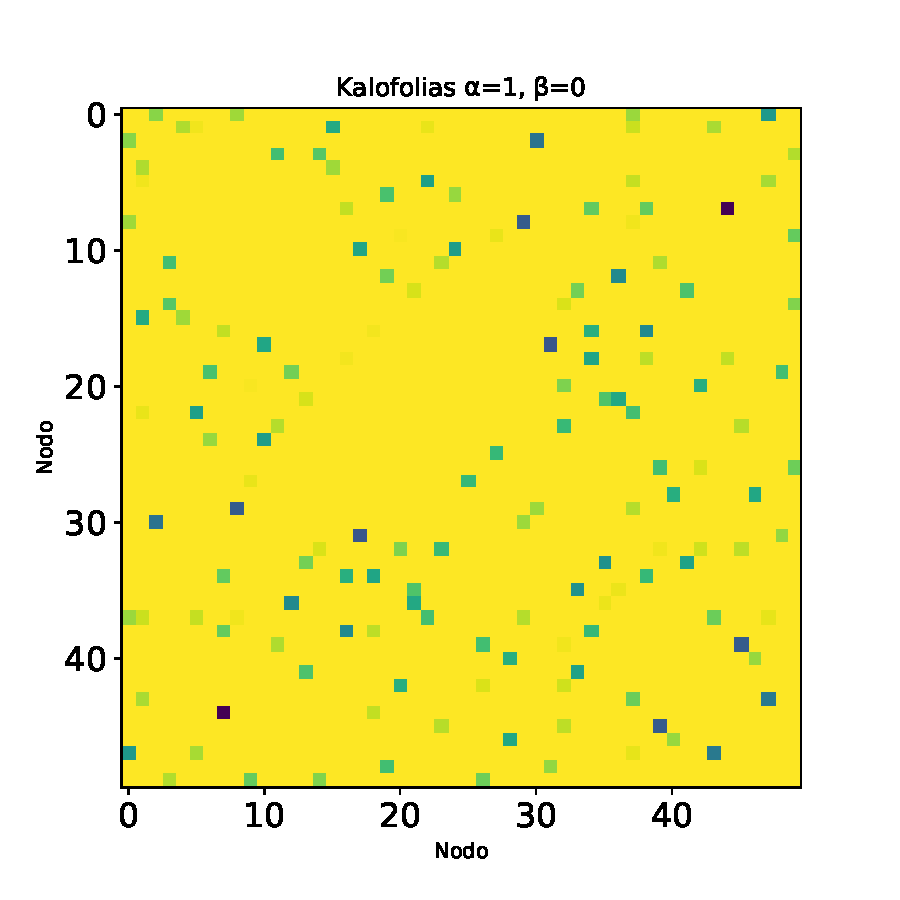
\includegraphics[width=0.28\textwidth]{imagenes/kalofolias/kalofolias_alpha1_beta0.pdf} &
            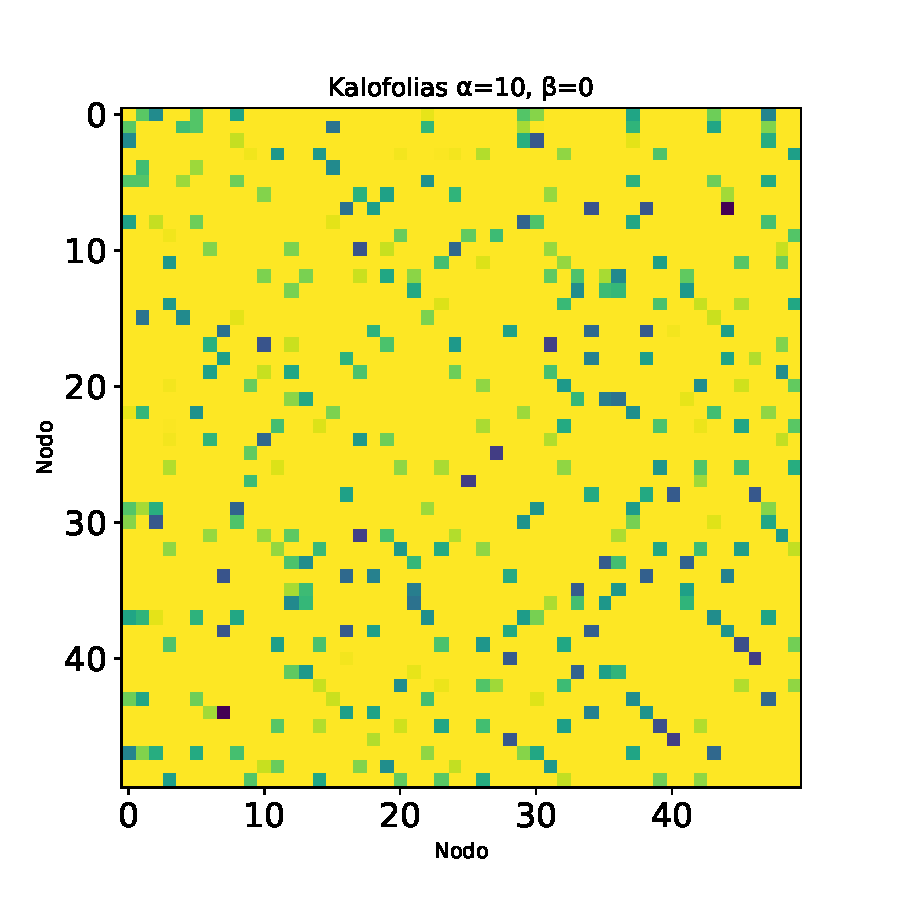
\includegraphics[width=0.28\textwidth]{imagenes/kalofolias/kalofolias_alpha10_beta0.pdf} \\
            $\alpha=0.1$, $\beta=0$ & $\alpha=1$, $\beta=0$ & $\alpha=10$, $\beta=0$ \\[1em]
            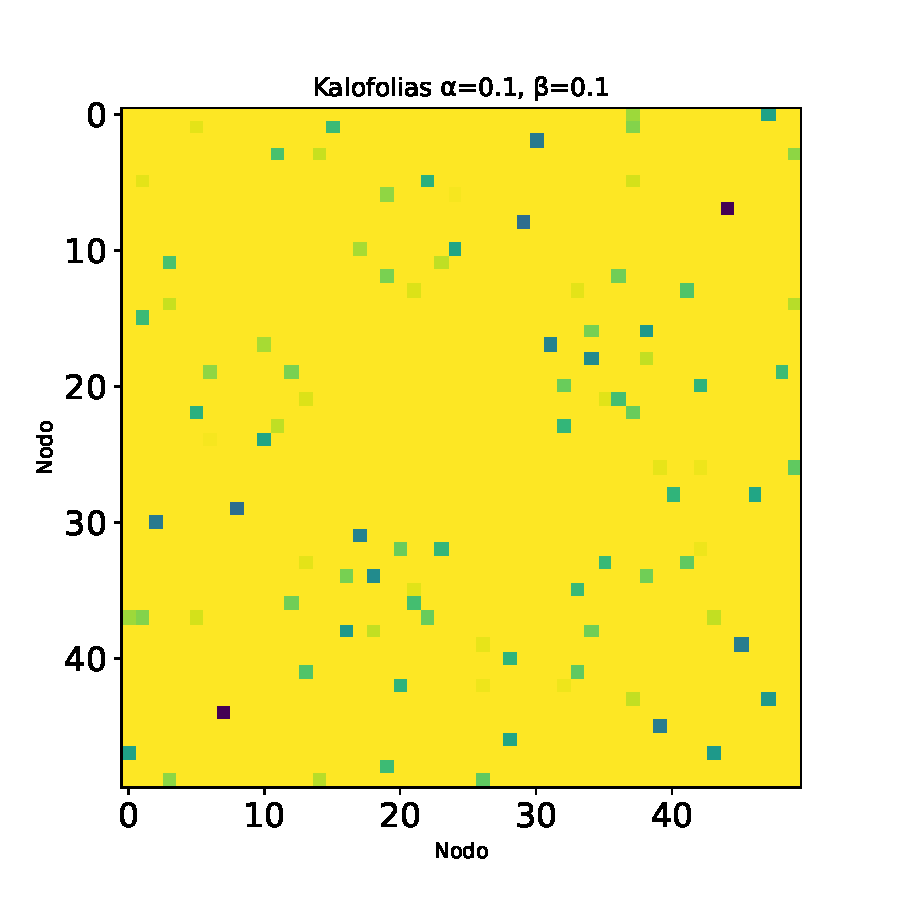
\includegraphics[width=0.28\textwidth]{imagenes/kalofolias/kalofolias_alpha0.1_beta0.1.pdf} &
            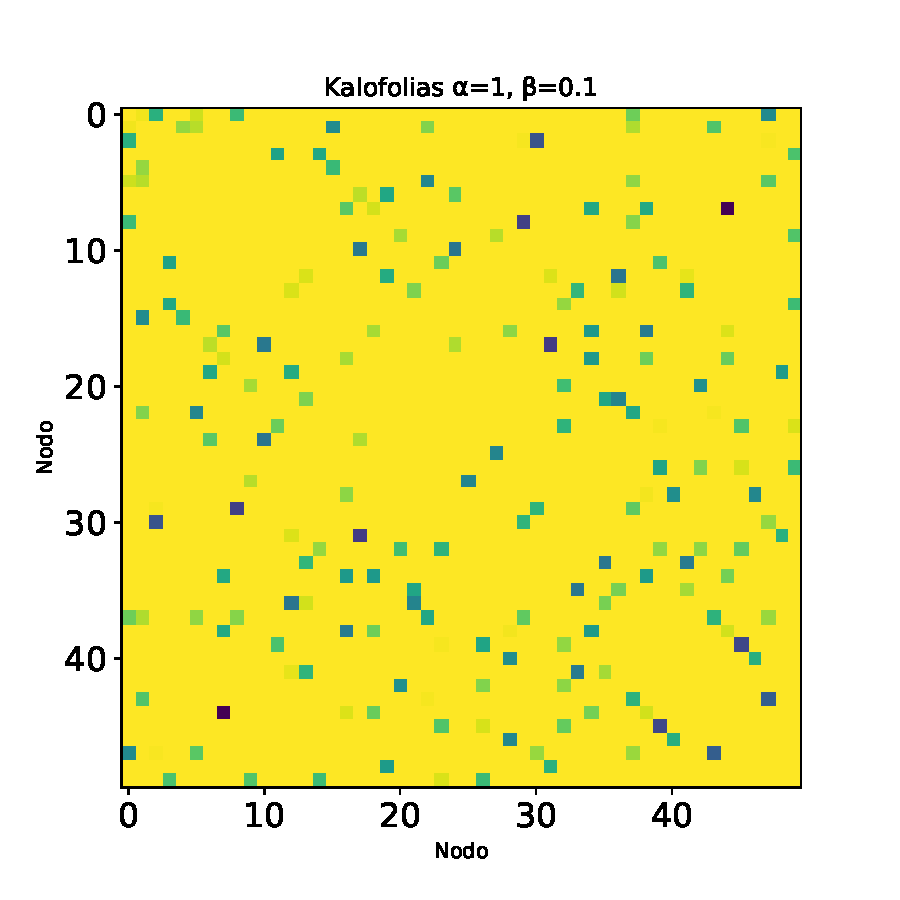
\includegraphics[width=0.28\textwidth]{imagenes/kalofolias/kalofolias_alpha1_beta0.1.pdf} &
            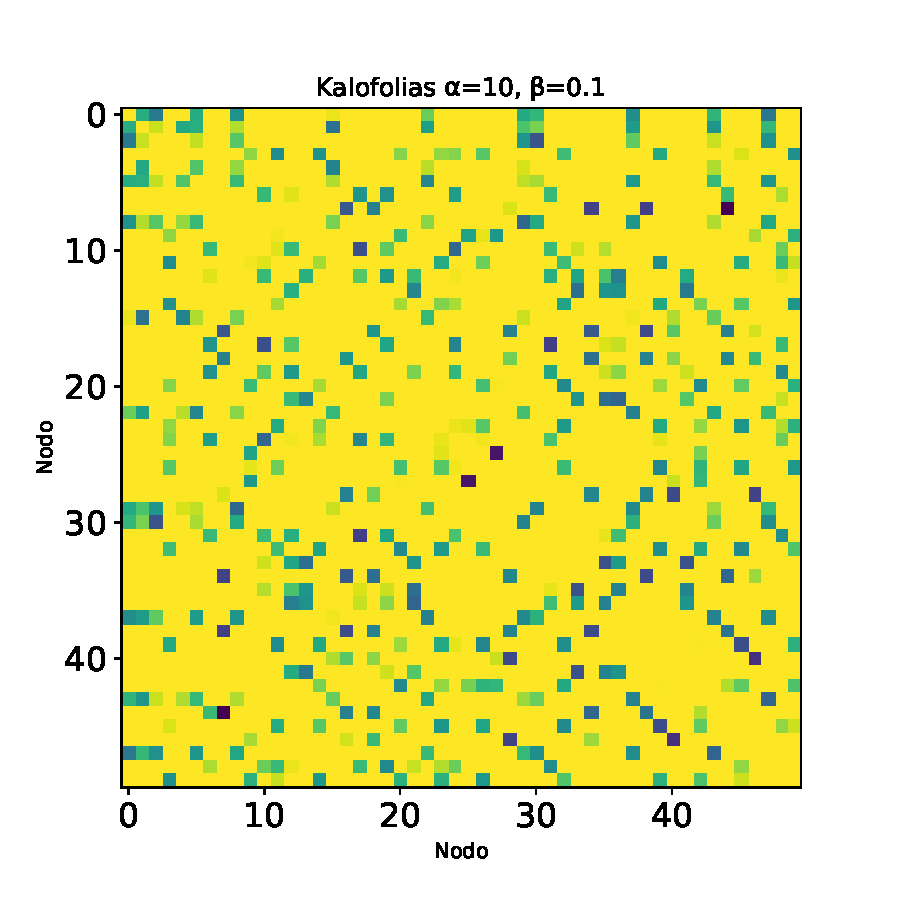
\includegraphics[width=0.28\textwidth]{imagenes/kalofolias/kalofolias_alpha10_beta0.1.pdf} \\
            $\alpha=0.1$, $\beta=0.1$ & $\alpha=1$, $\beta=0.1$ & $\alpha=10$, $\beta=0.1$ \\[1em]
            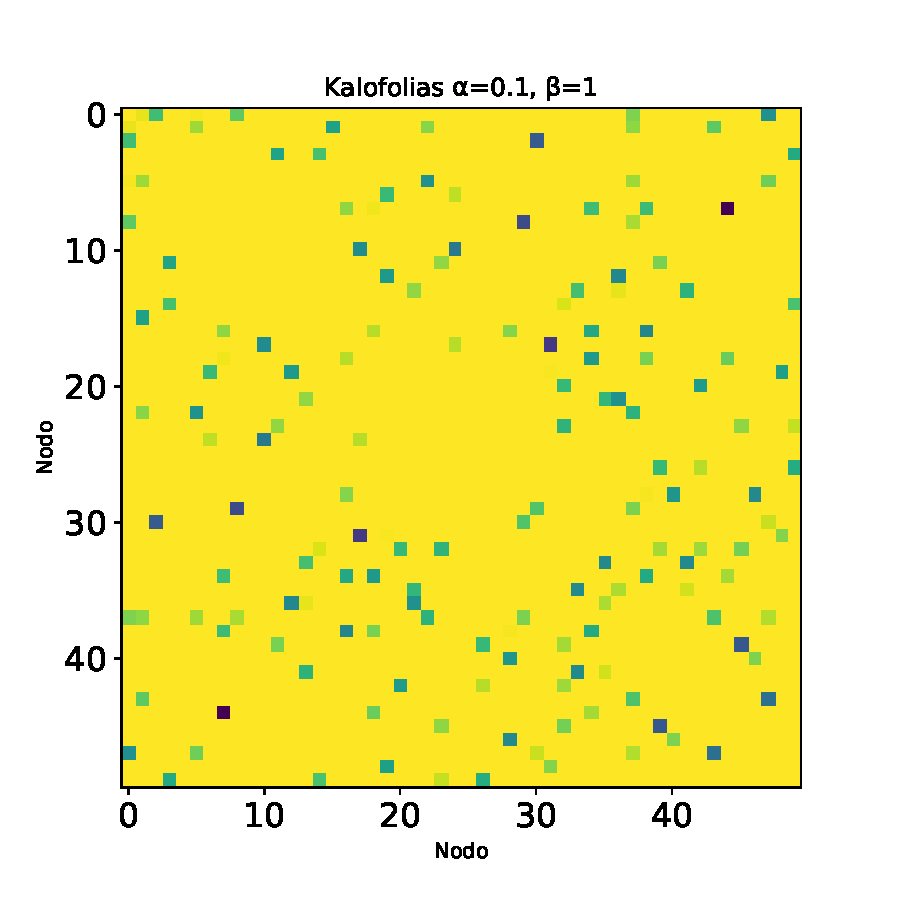
\includegraphics[width=0.28\textwidth]{imagenes/kalofolias/kalofolias_alpha0.1_beta1.pdf} &
            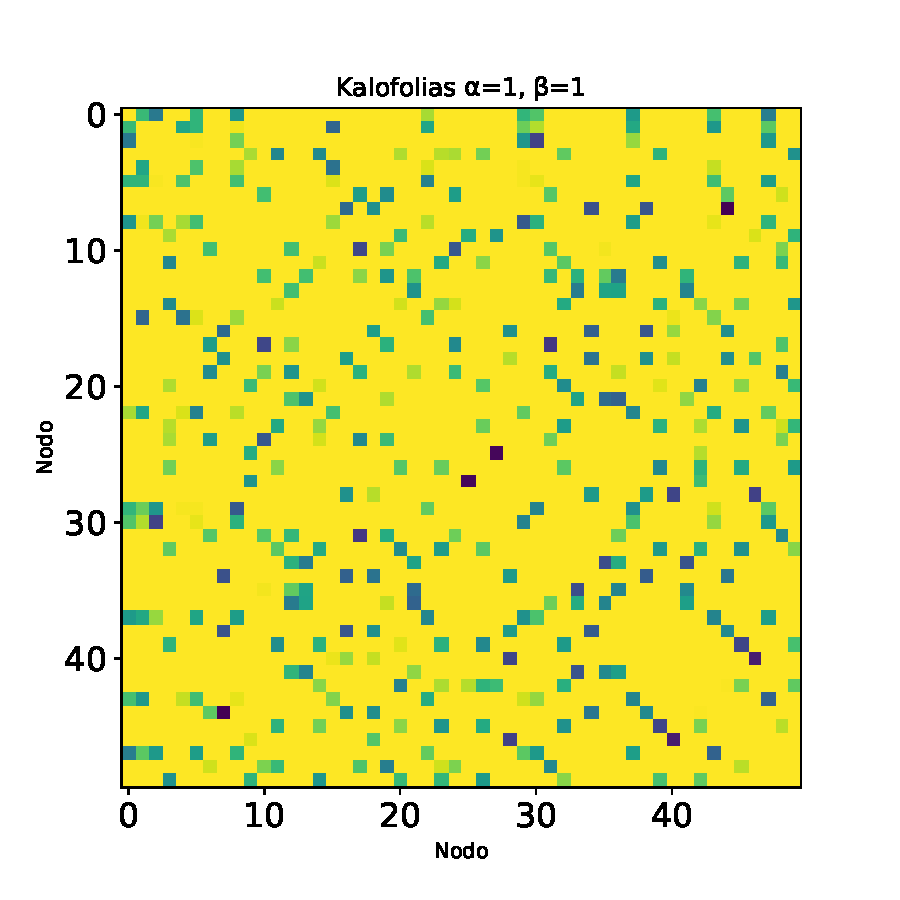
\includegraphics[width=0.28\textwidth]{imagenes/kalofolias/kalofolias_alpha1_beta1.pdf} &
            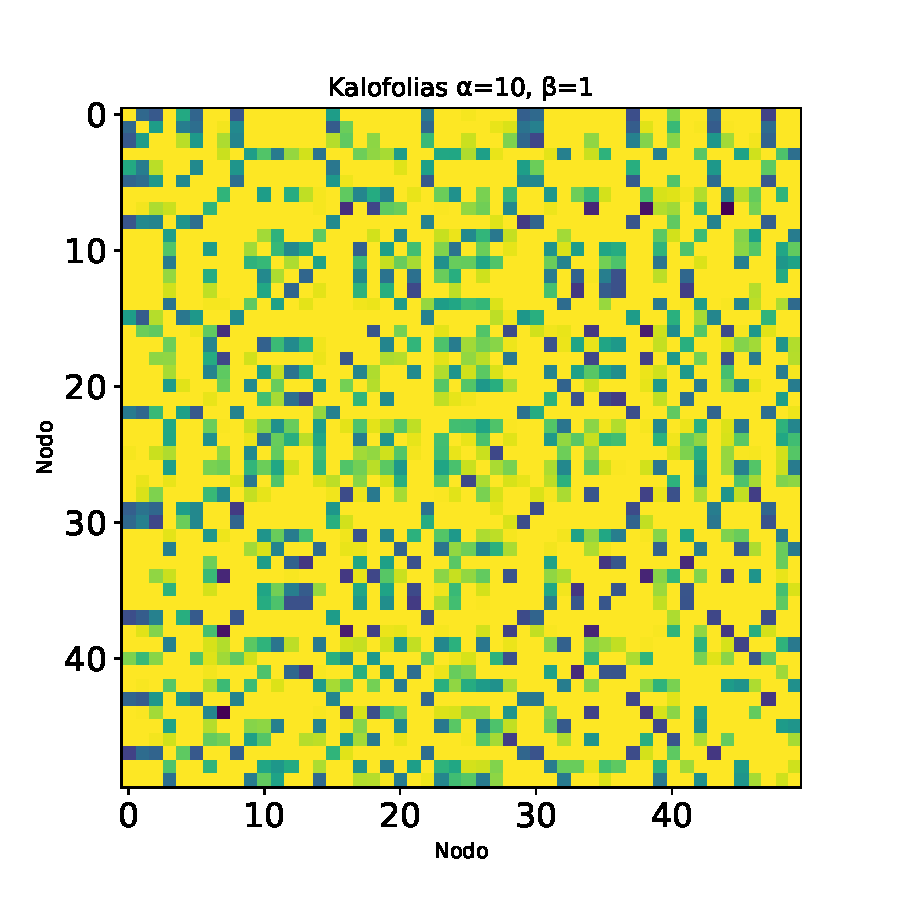
\includegraphics[width=0.28\textwidth]{imagenes/kalofolias/kalofolias_alpha10_beta1.pdf} \\
            $\alpha=0.1$, $\beta=1$ & $\alpha=1$, $\beta=1$ & $\alpha=10$, $\beta=1$ \\
        \end{tabular}
    \end{minipage}
    \caption{Resultados del método de Kalofolias para distintos valores de $\alpha$ y $\beta$, comparados con la matriz verdadera (izquierda) y una grilla 3x3 de variaciones (derecha).}
    \label{fig:kalofolias_grid}
\end{figure}


\subsection{Comparación y visualización de los grafos aprendidos}

En la figura \ref{fig:generated_graphs_syntetic} se presenta una comparación visual entre el grafo verdadero y los grafos aprendidos mediante los métodos de Graphical Lasso, Meinshausen y Bühlmann, y Kalofolias. Cada subfigura muestra la estructura de conexiones entre nodos, permitiendo observar las similitudes y diferencias en la topología inferida por cada método en relación con el grafo original.

\begin{figure}[htb]
    \centering
    \begin{subfigure}[t]{0.24\linewidth}
        \centering
        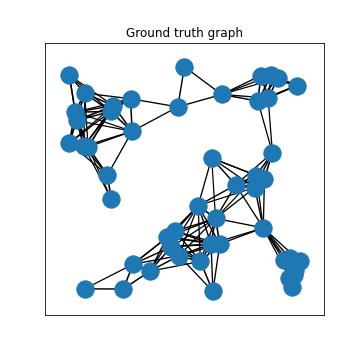
\includegraphics[width=\textwidth]{imagenes/generated_graph_syntetic/ground_truth_graph.png}
        \caption{Grafo verdadero}
    \end{subfigure}\hfill
    \begin{subfigure}[t]{0.24\linewidth}
        \centering
        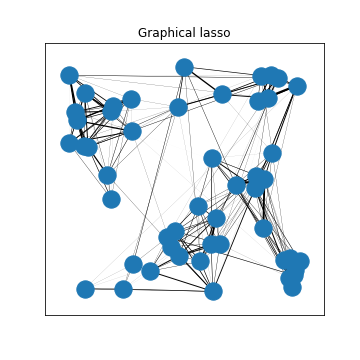
\includegraphics[width=\textwidth]{imagenes/generated_graph_syntetic/graphical_lasso.png}
        \caption{Graphical Lasso}
    \end{subfigure}\hfill
    \begin{subfigure}[t]{0.24\linewidth}
        \centering
        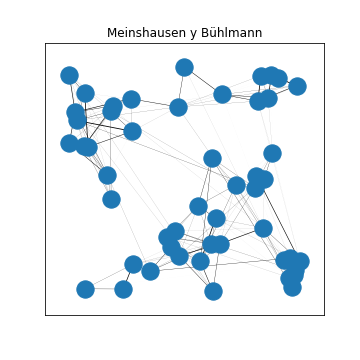
\includegraphics[width=\textwidth]{imagenes/generated_graph_syntetic/meinshausen_buhlmann.png}
        \caption{Meinshausen y Bühlmann}
    \end{subfigure}\hfill
    \begin{subfigure}[t]{0.24\linewidth}
        \centering
        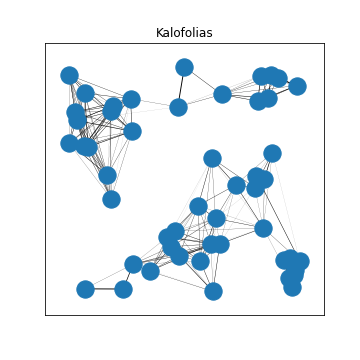
\includegraphics[width=\textwidth]{imagenes/generated_graph_syntetic/kalofolias.png}
        \caption{Kalofolias}
    \end{subfigure}
    \caption{Comparación visual de los grafos: verdadero y aprendidos por distintos métodos.}
    \label{fig:generated_graphs_syntetic}
\end{figure}
La comparación visual de la figura~\ref{fig:generated_graphs_syntetic} muestra que Graphical Lasso recupera bien la estructura principal del grafo, aunque introduce algunas conexiones espurias; Meinshausen y Bühlmann produce un grafo más disperso, capturando solo las conexiones más fuertes y perdiendo muchas débiles; y Kalofolias logra un balance intermedio, con una topología similar pero no idéntica al grafo original. 


\section{Inferencia de topología en MNIST}
\label{sec:mnist}
Para esta parte trabajaremos el dataset MNIST, que contiene imágenes de dígitos escritos a mano. El objetivo es aprender la estructura del grafo que conecta las imágenes basándonos en sus características visuales, y luego utilizar esta estructura para realizar clustering espectral y evaluar su desempeño.

\subsection{Descripción del dataset y preprocesamiento}
Para trabajar, nos quedaremos con un subconjunto de 2000 imágenes (doscientas por cada dígito) de dimensión $28 \times 28$ píxeles. Cada imagen la convertimos en un vector de dimensión 784 (aplanando la matriz) y normalizamos los valores de píxeles al rango $[0,1]$. 

Para dimensionar la dificultad del problema, se realiza un análisis preliminar utilizando t-SNE para reducir la dimensionalidad de los datos a 2D y visualizar la distribución de las imágenes. En la figura~\ref{fig:tsne_mnist} se observa que los dígitos forman grupos relativamente bien definidos, aunque con cierta superposición, y algunas muestras quedan lejos de su respectivo grupo (\textit{outliers}) lo que indica que el clustering no será trivial.

\begin{figure}[htb]
    \centering
    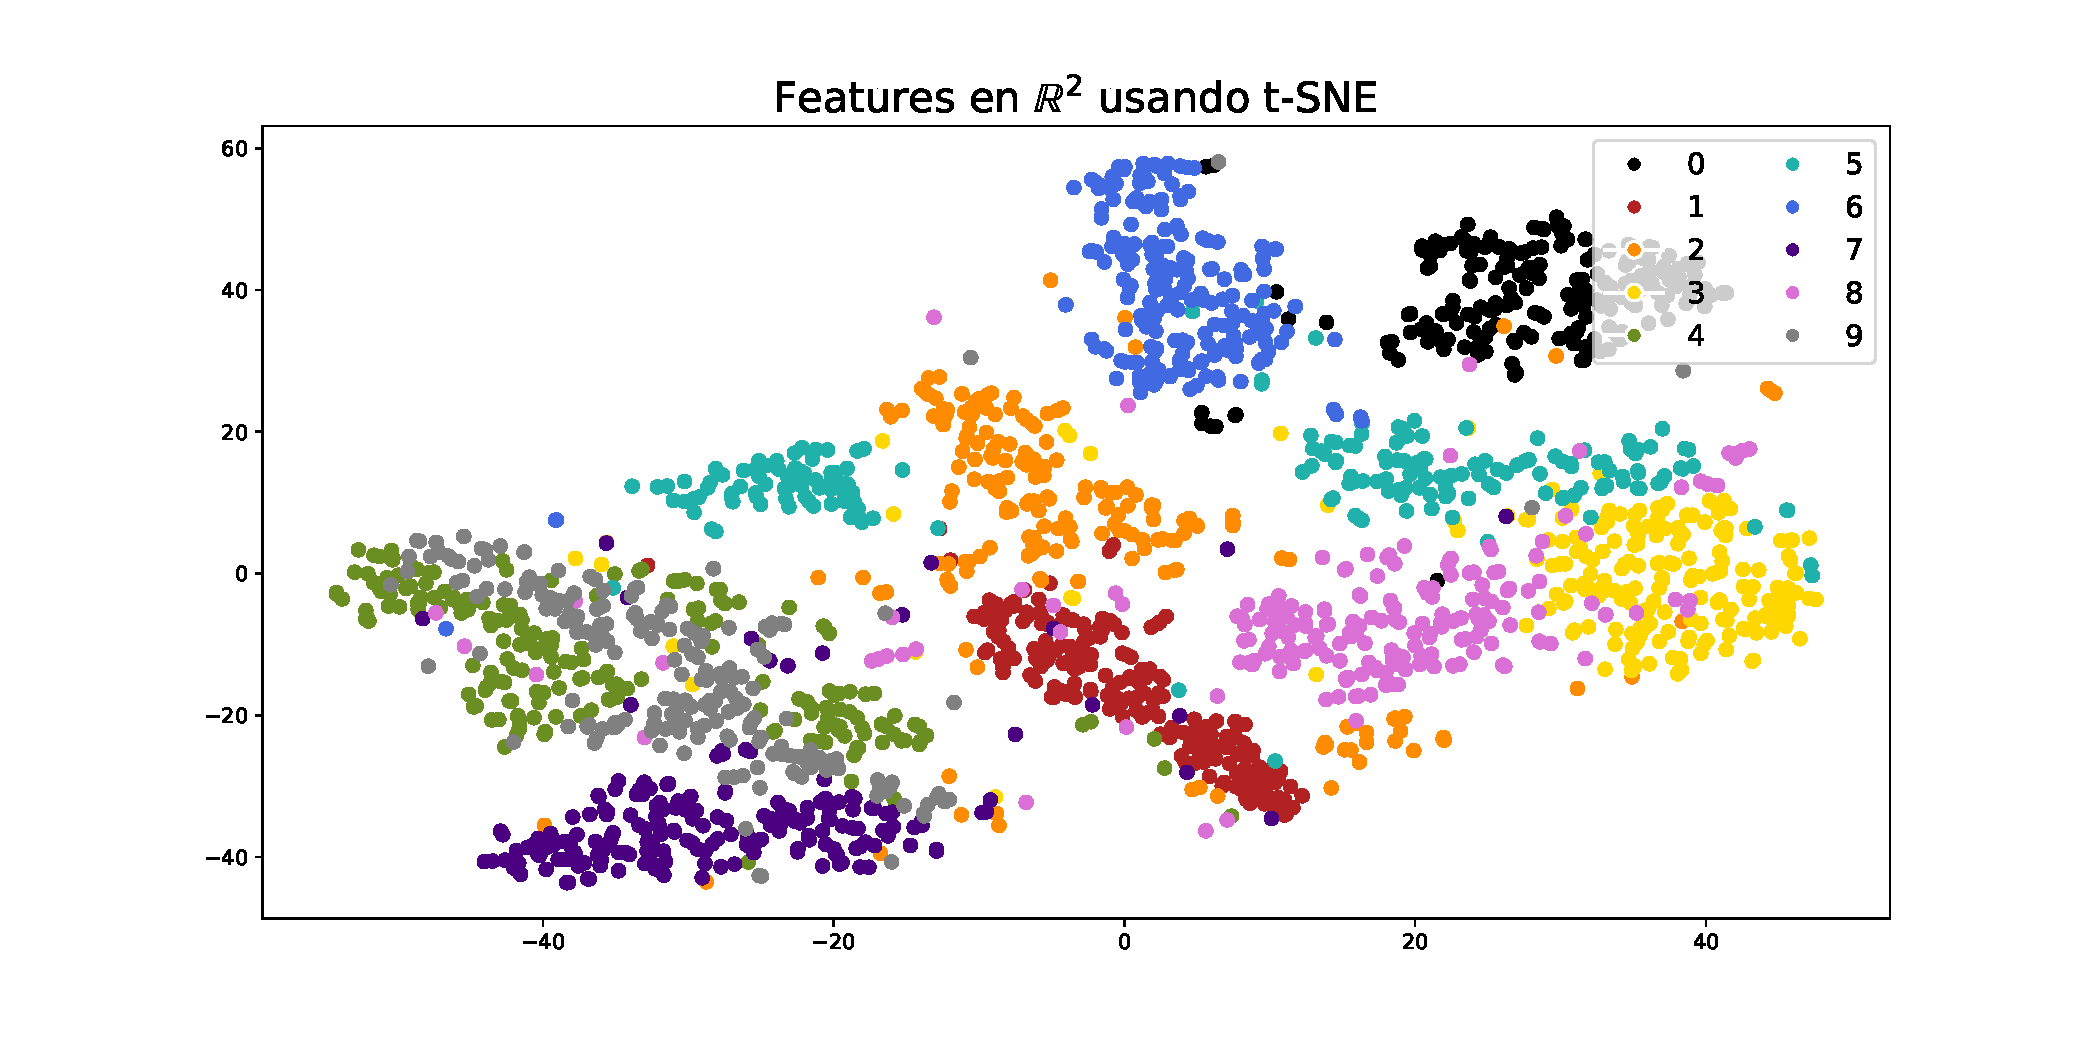
\includegraphics[width=0.8\textwidth]{imagenes/mnist/tsne_mnist.pdf}
    \caption{Visualización t-SNE del subconjunto de 2000 imágenes del dataset MNIST.}
    \label{fig:tsne_mnist}
\end{figure}   

Se trabajará con cada imagen como un nodo del grafo, y se buscará aprender las conexiones entre ellas basándose en si son similares en algún sentido.


\subsection{Grafo aprendido con Meinshausen y Bühlmann}

Utilizando el método de Meinshausen y Bühlmann implementado previamente, aprendemos la estructura del grafo a partir de las imágenes del dataset MNIST. Se muestra en la figura ~\ref{fig:mnist_meinshausen} el grafo resultante. Cada dígito se representa como un subgrafo circular para facilitar la visualización. Se puede ver que dentro de cada subgrafo los nodos están densamente conectados, reflejando la similitud entre imágenes del mismo dígito. Además, hay conexiones entre diferentes dígitos, lo que indica que algunas imágenes comparten características visuales a pesar de pertenecer a clases distintas. Por ejemplo, se puede ver una fuerte tendencia a conectar los dígitos 4 y 9 o el 3 y el 8. 
\begin{figure}[htb]
    \centering
    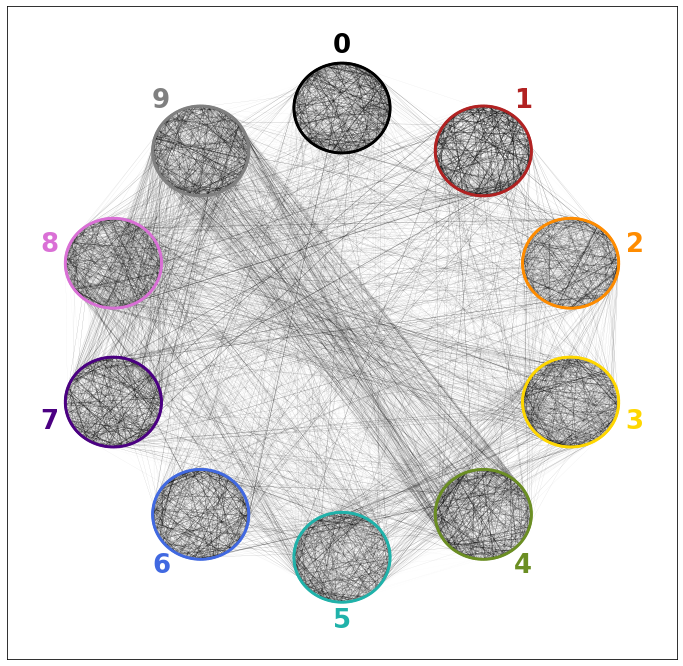
\includegraphics[width=0.6\textwidth]{imagenes/mnist/grafo_meinshausen_mnist.png}
    \caption{Grafo aprendido con el método de Meinshausen y Bühlmann sobre el dataset MNIST.}
    \label{fig:mnist_meinshausen}
\end{figure}

\subsection{Grafo aprendido con Kalofolias y umbralización}
Realizamos el aprendizaje del grafo utilizando el método de Kalofolias. Dado que este método produce una matriz de adyacencia densa, aplicamos una umbralización para eliminar las conexiones más débiles y obtener un grafo más interpretable. En la figura~\ref{fig:mnist_kalofolias} se muestra el grafo resultante tras aplicar Kalofolias y umbralizar los pesos de las aristas. Se puede observar que para cada dígito, los nodos están fuertemente conectados (se distinguen subgrafos más densos en comparación con el método anterior). Sin embargo, la tendencia a conectarse entre dígitos distintos todavía se mantiene fuerte para el caso entre el 4 y 9.  

\begin{figure}[htb]
    \centering
    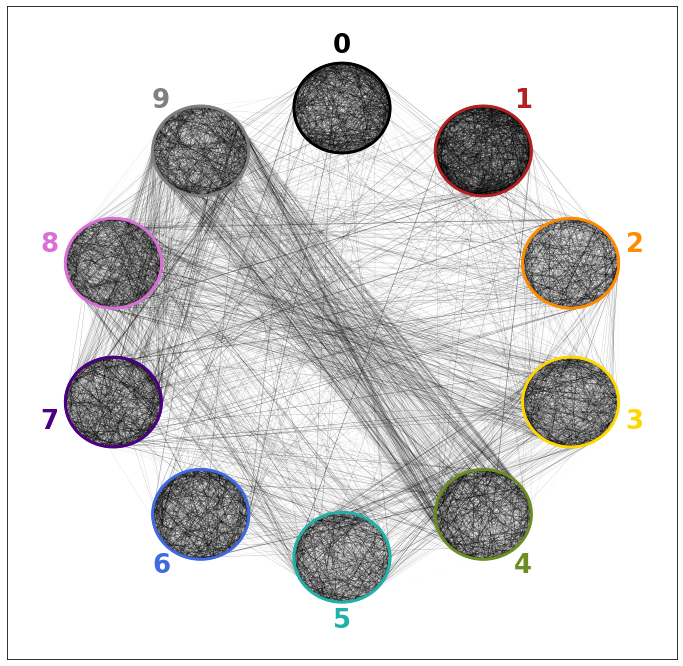
\includegraphics[width=0.6\textwidth]{imagenes/mnist/grafo_kalofolias_mnist.png}
    \caption{Grafo aprendido con el método de Kalofolias y umbralización sobre el dataset MNIST.}
    \label{fig:mnist_kalofolias}
\end{figure}

\subsection{Clustering espectral sobre grafos aprendidos}

Una vez obtenidos los grafos mediante los diferentes métodos de aprendizaje, aplicamos clustering espectral para agrupar las imágenes y evaluamos su desempeño utilizando métricas estándar. Los resultados se presentan en la tabla~\ref{tab:clustering_results}, donde se comparan las diferentes estrategias de aprendizaje de grafos junto con el clustering en el espacio original y con representación t-SNE.

\begin{table}[htb]
\centering
\begin{tabular}{lccc}
\hline
\textbf{Método} & \textbf{V-Measure} & \textbf{Rand} & \textbf{Fowlkes-Mallows} \\
\hline
Clustering en espacio original & 0.608977 & 0.414621 & 0.487145 \\
Meinshausen & 0.591794 & 0.322577 & 0.432388 \\
Kalofolias & 0.704810 & 0.484090 & 0.562653 \\
Clustering con t-SNE & 0.627884 & 0.475135 & 0.532973 \\
\hline
\end{tabular}
\caption{Resultados de clustering espectral para diferentes métodos de aprendizaje de grafos evaluados con métricas V-Measure, Rand Index y Fowlkes-Mallows.}
\label{tab:clustering_results}
\end{table}

Los resultados muestran que el método de Kalofolias obtiene el mejor desempeño en todas las métricas evaluadas, superando incluso al clustering en el espacio original y con t-SNE. El método de Meinshausen y Bühlmann presenta el desempeño más bajo, lo que sugiere que la estructura de grafo aprendida por este método no captura adecuadamente las relaciones relevantes para el clustering de dígitos. El clustering con t-SNE logra un desempeño intermedio, confirmando que la reducción de dimensionalidad mejora la separabilidad de los grupos pero sin alcanzar los resultados del método de Kalofolias.

\subsection{Visualización en el plano t-SNE por método}
Para visualizar cómo los diferentes métodos de aprendizaje de grafos afectan la distribución de las imágenes en el espacio reducido, aplicamos t-SNE a las representaciones obtenidas por cada método. En la figura~\ref{fig:tsne_by_method} se presentan las visualizaciones t-SNE correspondientes a cada enfoque.

\begin{figure}[htb]
    \centering
    \begin{minipage}[t]{0.45\textwidth}
        \vspace{0pt}
        \centering
        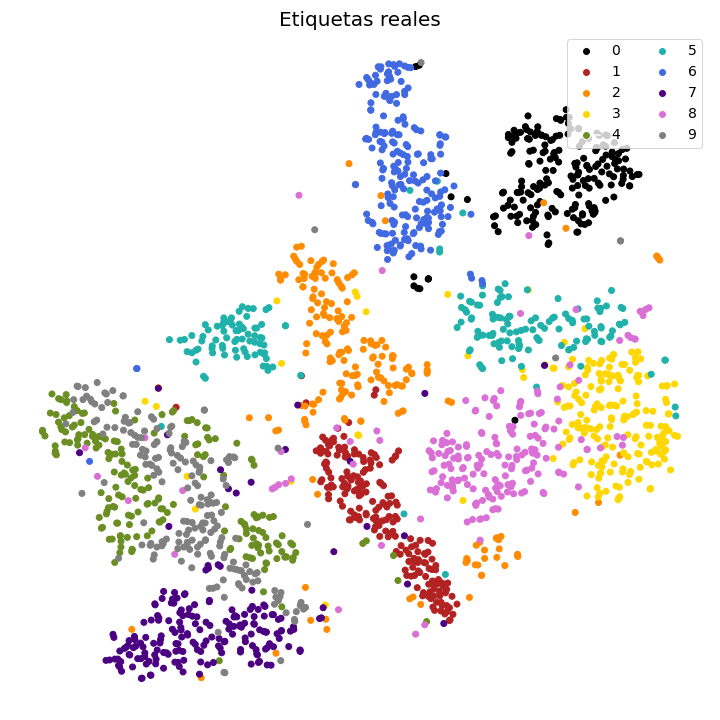
\includegraphics[width=\textwidth]{imagenes/mnist/mnist_real_labels.png}
        \caption*{Etiquetas reales}
    \end{minipage}
    \hfill
    \begin{minipage}[t]{0.53\textwidth}
        \vspace{0pt}
        \centering
        \begin{tabular}{cc}
            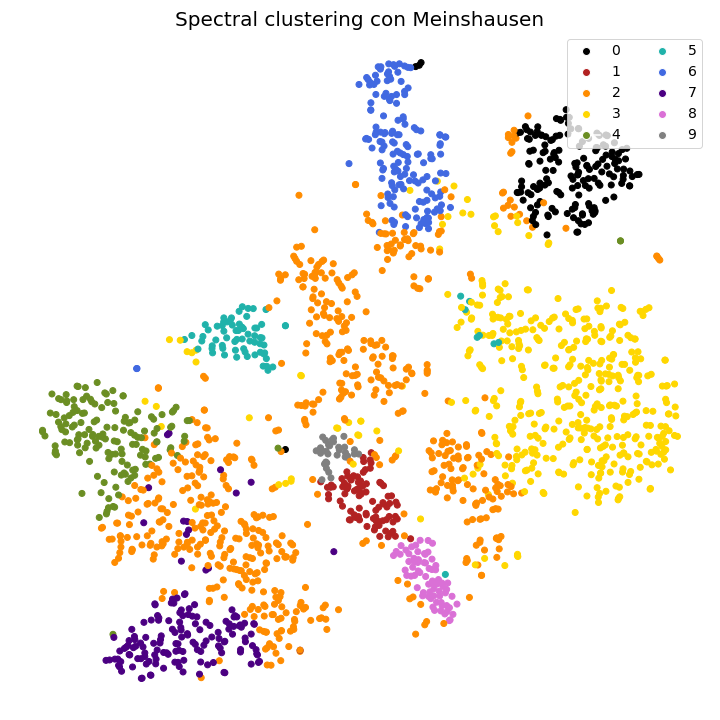
\includegraphics[width=0.48\textwidth]{imagenes/mnist/mnist_clustering_meinshausen.png} &
            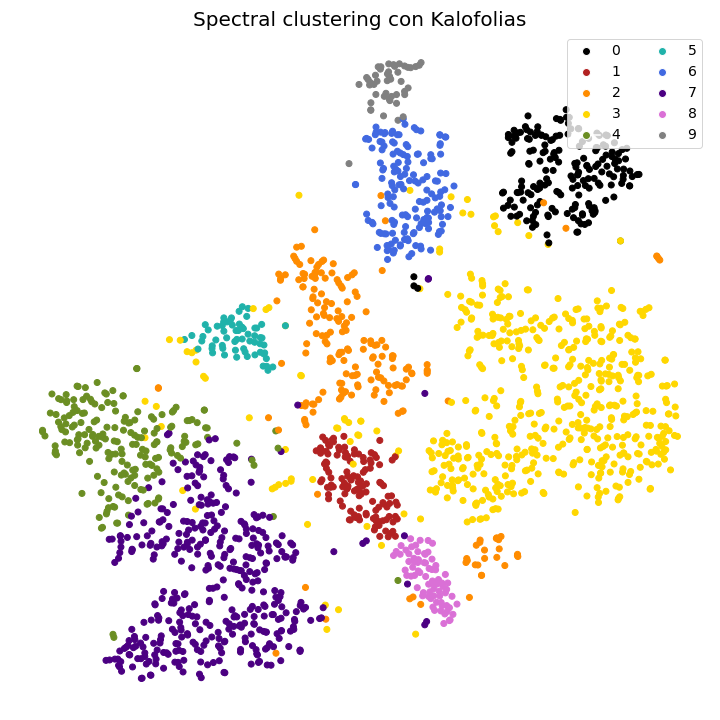
\includegraphics[width=0.48\textwidth]{imagenes/mnist/mnist_clustering_kalofolias.png} \\
            Meinshausen & Kalofolias \\
            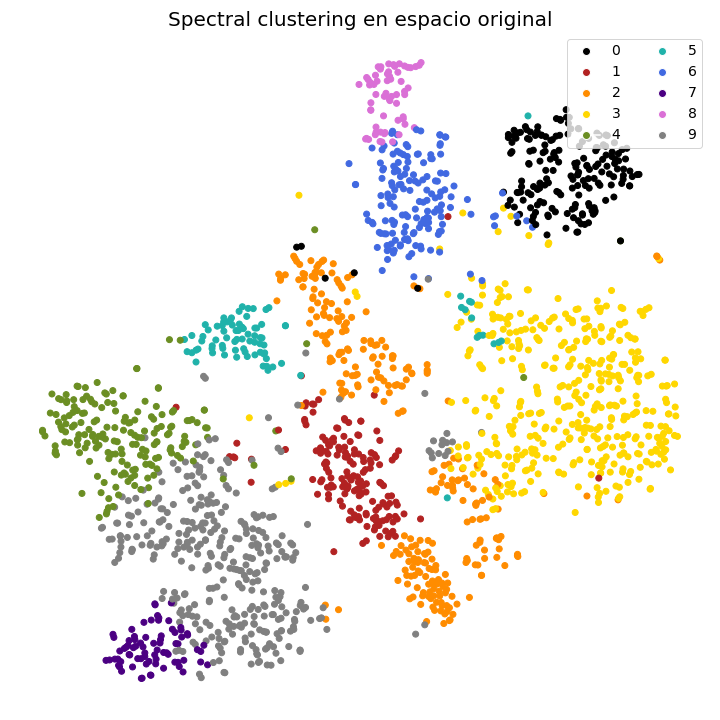
\includegraphics[width=0.48\textwidth]{imagenes/mnist/mnist_clustering_original.png} &
            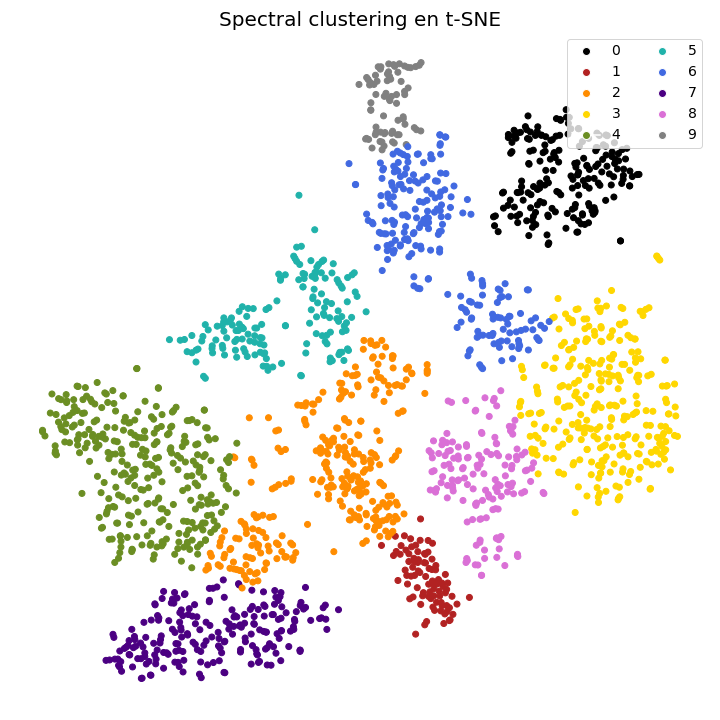
\includegraphics[width=0.48\textwidth]{imagenes/mnist/mnist_clustering_tsne.png} \\
            Espacio original & t-SNE \\
        \end{tabular}
    \end{minipage}
    \caption{Visualización t-SNE de las imágenes MNIST. Izquierda: etiquetas reales. Derecha: resultados de clustering espectral usando los grafos aprendidos por cada método y en el espacio original.}
    \label{fig:tsne_by_method}
\end{figure}

Analizando las diferencias entre el método de Kalofolias y el clustering con t-SNE, lo primero que salta a la vista es que Kalofolias logra correctamente muestras que se encuentran más aisladas de su cluster principal, mientras que t-SNE asigna clusters más compactos perdiendo las muestras atípicas. Esto sugiere que Kalofolias es más robusto a la presencia de \textit{outliers} y puede capturar mejor la variabilidad dentro de cada clase. 



% \section{Referencias}
\bibliographystyle{plain}
\bibliography{refs}


\end{document}